\section{Baseline method}
\label{sec:baseline}

\begin{figure}
\centering
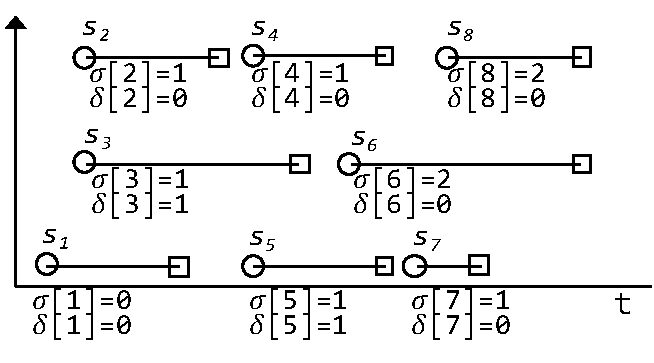
\includegraphics[width=2.5in]{figs/stabarray.pdf}
\caption{Stabbing count array for $I$ from Figure~\ref{example}.}
\label{fig:stabarray}
\end{figure}

Le et al.~\cite{Le2013} provide a centralized greedy algorithm for
optimal splitters where optimality is defined as above.  The algorithm
has two parts: a) compute a stabbing count array equal in size to
input size N; b) use binary search to find the smallest partition cost
which yeilds up to $k$ splitters.

{\bf A. Stabbing count array.}  The stabbing count array contains two
values for each input interval: the number of intervals that strongly
cover (contain) the start value of $i$ $\sigma(i) = |I^x(s_i)|$ and
the number of intervals with the same start value as $i$ that precede
it $\delta(i) = |I^o_<(s_i)|$.  Figure~\ref{fig:stabarray}
demonstrates this on our running example.

To construct the stabbing count array, the start and end points of the
input array are sorted in increasing order and then a single
sequential pass computes the $\sigma$ and $\delta$ values for each
interval as shown in Algorithm~\ref{alg:stabbingcount}.

\begin{algorithm}
\caption{StabbingCount(I)}
\begin{algorithmic}[1]
\State $P \gets (I.s,I.s) \cup (I.e,I.s) $\Comment{union of all start and end points of I with their associated start points}
\State $E \gets sort(P)$\Comment{sort in increasing order, break ties by start}
\State $c \gets 0; c_\delta \gets 0; s_{last} \gets -\infty; i \gets 1$
\For{$j \gets 1, \ldots, 2N$}
\If {$E(j)._1 =  E(j)._2$}\Comment{starting value}
\State $c \gets c + 1$
\If {$E(j)._1 = s_{slast}$}
\State $c_{\delta} \gets c_{\delta} + 1$
\Else
\State $s_{last} \gets E(j)._1$
\State $c_{\delta} \gets 1$
\EndIf
\State $A(i) \gets (c - c_{\delta}, c_{\delta} - 1)$
\State $i \gets i + 1$
\Else \Comment{ending value} %{$E(j)._1 = \text{ending value}$}
\State $c \gets c - 1$
\If {$s_{last} = E(j)._2$}
\State $c_{\delta} \gets c_{\delta} - 1$
\EndIf
\EndIf
\EndFor
\Return $A$
\end{algorithmic}
\label{alg:stabbingcount}
\end{algorithm}

As shown in the paper, the work of this step is $\Theta(N~log~N)$ for
the sort and $\Theta(N)$ for the sweep, resuling in $O(N~log~N)$.  In
a centralized environment the span (depth) of this algorithm is the
same as its work, i.e. $O(N~log~N)$.  However, we can trivially use
parallelized sort which does not change $W$ but reduces the span to
$\Theta(log^2 N) + \Theta(N) = O(N)$ and improves parallelism to
$O(log~N)$.

{\bf B. Binary search on $t$.}  Given a stabbing count array, Le et
al. formulate the problem of finding the optimal splitters as a
repeated decision problem.  Given input $k$, we find the smallest cost
$t$ that produces a valid $P(k,I)$ using repeated invocations of
Algorithm~\ref{alg:tjump}, reproduced here for the reader, with
different values of $t$ determined by a binary search.

\begin{algorithm}
\caption{t-jump(I,k,t)}
\begin{algorithmic}[1]
\If {$t \geq N$}
\Return $\overline{t} = N$, and an empty splitter set
\EndIf
\State $p(1) \gets t + 1 - \delta[t+1]; |b_1| \gets t - \delta[t+1]$
\If {$|b_1| = 0$}
\Return $\overline{t} = |b_1|$
\EndIf
\State $\overline{t} = |b_1|$
\For{$j \gets 2,\ldots,k$}
\State $x_j \gets p(j-1) + t - \sigma[p(j-1)]$
\If {$x_j > N$}
\State $|b_j| \gets N - p(j-1) + 1 + \sigma[p(j-1)]$
\State $\overline{t} \gets max(\overline{t}, |b_j|)$
\State \Return $\overline{t}$, and splitters $s_{p(1)}, \ldots, s_{p(j-1)}$
\EndIf
\State $p(j) \gets x_j - \delta[x_j]$
\If {$p(j) = p(j-1)$}
\Return $\overline{t} \gets 0$
\EndIf
\State $|b_j| \gets t - \delta[x_j]; \overline{t} \gets max(\overline{t}, |b_j|)$
\EndFor
\State $|b_{k+1}| = N - p(k) + 1 + \sigma[p(k)]$
\If {$|b_{k+1}| > t$}
\Return $\overline{t} \gets 0$
\EndIf
\State $\overline{t} = max(\overline{t}, |b_{k+1}|)$
\State \Return $\overline{t}$, and splitters $s_{p(1)}, \ldots, s_{p(k)}$
\end{algorithmic}
\label{alg:tjump}
\end{algorithm}

The cost of finding a solution for a given $k$ is $O(k ~log ~N)$ using
binary search of on different values of cost.  This is a sequential
algorithm, so the span is also $O(k~log~N)$ and thus parallelism is
$P(N) = O(1)$.

Le et al. also provide a concurrent t-jump algorithm that improves the
performance of part B by evaluating $h$ multiple values of
candidate cost in parallel.  $W(N) = \Theta(log_hN*hk)$, $S(N) =
\Theta(log_hN)$, which leads to $P(N) = O(hk)$.

Putting parts A and B together, Le et al. provide a solution to the
optimal splitters problem with $O(N~log~N)$ work and $O(log~N)$ span.
As we show in the next section, we can achieve better parallelism for
this problem with the same asymptotic work.


